\subsection{Interface}
    These are the server side scripts that will be used across the website.

    \emph{Constants}
    \begin{itemize}
        \item `header.php'
        \item `footer.php'
        \item `config.php'
        \item \$title   
        \item config.php
        \begin{itemize}
            \item \$CONFIG
        \end{itemize}

        \item Index
        \begin{itemize}
            \item \$title
            \item include `header.php';
            \item include `config.php';
            \item text
            \begin{itemize}
                \item app link
            \end{itemize}
            \item include `footer.php';
        \end{itemize}

        \item About
        \begin{itemize}
            \item \$title
            \item include `header.php';
            \item include `config.php';
            \item text
            \begin{itemize}
                \item app link
            \end{itemize}
            \item include `footer.php';
        \end{itemize}       

        \item reserves
        \begin{itemize}
            \item include `config.php';
            \item \$title
            \item include `header.php';
            \item include `reserves\_curl';
            \item form(GET)
            \item include `footer.php';
        \end{itemize}
        
        \item add\_reserve
        \begin{itemize}
            \item include `config.php';
            \item \$title
            \item include `header.php';
            \item form(input)
            \item include `footer.php';
        \end{itemize}
        
        \item edit\_reserve
        \begin{itemize}
            \item include `config.php';
            \item \$title
            \item include `header.php';
            \item include `get\_reseve.php';
            \item form(input)
            \item include `footer.php';
        \end{itemize}
        
        \item specimen
        \begin{itemize}
            \item include `config.php';
            \item \$title
            \item include `header.php';
            \item include `specimens\_curl.php';
            \item include `filter.php';
            \item map pop-up
            \item include `footer.php';
        \end{itemize}
        
        \item add\_specimen
        \begin{itemize}
            \item include `config.php';
            \item \$title
            \item include `header.php';
            \item form(input)
            \item if no image uploaded, default image else uploaded image
            \item include `footer.php';
        \end{itemize}
        
        \item edit\_specimen
        \begin{itemize}
            \item include `config.php';
            \item \$title
            \item include `header.php';
            \item include `record\_curl.php';
            \item form(input)
            \item if no image uploaded, default image else uploaded image
            \item include `footer.php';
        \end{itemize}
        
        \item plant\_specimens
        \begin{itemize}
            \item include `config.php';
            \item \$title
            \item include `header.php';
            \item include `specimens\_curl.php';
            \item include `filter.php';
            \item form(input)
            \item include `footer.php';
        \end{itemize}
    \end{itemize}


\subsection{Detailed design}

    \subsubsection{index.php}
        This is the front page of the website to the user, it contains a description of the purpose of the site.

        
    \subsubsection{about.php}
        This page contains a short description about the app as well as the team.

        
    \subsubsection{reserves.php}
        This page contains a script to display the data from the json object for the reserves. It includes scripts to retrieve the json oject as well as to delete the json ojects.

        
    \subsubsection{add\_reserve.php}
        The page gives the user the ability to input data for a new reserve in to a html form. This page also contains a script to collect the data into a json object and a curl method to send the json object to the server.

        
    \subsubsection{edit\_reserve.php}
        Edit reserve returns the contents of a json object for reserve to a html form allowing the user to edit its details. A script to encode the reserve to a json object is also included in the page as well as a curl methodto send the json object to the server.

        
    \subsubsection{specimen.php}
        Specimen has a script to return the data from the json object to a table to display as a friendly interface to the user. There is scripts for navigation within the record, these create links to the next and previous specimens within the record. There is a script within the page which produces a pop-up map (using google maps) displaying the location of where this specimen was found. This page also contains scripts to include the site and specimen images.

        
    \subsubsection{add\_specimen.php}
        This page contains a html form to collect data from the user about a new specimen to be added. The page also contains a script to make the data into a new json object as well as a curl method to send the data to the server. There is a script to upload images which are then sent to a private folder via a curl method.

        
    \subsubsection{edit\_specimen.php}
        Edit specimen contains a script to retrieve the data from the specimen json object and places it in to a html form for the user to edit. There is also scripts to encode the edited data to a json object and to submit the object to the server via a curl method.

        
    \subsubsection{plant\_specimens.php}
        Plant specimens contains a script which allows the user to search the database to find a specific species. This page also contains 


    \subsubsection{config.php}
        The config.php file will be used to establish the connection to the mysql database using the servers API at the start of a new session.
        \begin{verbatim}
            $CONFIG=array
            api="file location"
            session="where the session is stored"
        \end{verbatim}
        The config.php will need to be be included in all php scripts.


    \subsubsection{authenticate.php}
        The authenticate.php script will be used to authenticate an admin user on the site. Who through entering a correct password will have access to certain features of the site that regular users will not have. Such as deletion of reserves and specimens. The authentication will be checked to the servers API. If a correct password is entered then the user will see a message confirming it. If an incorrect password is used then a different message will be see saying that a wrong password has been used.


    \subsubsection{delete\_curl.php}
        This script is used to delete specific specimens from the servers database. This feature will only become available once a user has entered a correct password to show that they are an admin user. PHP CURL is used so that the website can communicate with the server.


    \subsubsection{edit\_specimens.php}
        This script is similar to the delete script. It uses PHP CURL to communicate with the server. This function is also only available to admin users.


    \subsubsection{footer.php}
        This script will be included on every page. It will contain a small website logo in the centre of the footer. 


    \subsubsection{get\_reseve.php}
        This will be used to call all the data about the reserves stored on the server. PHP CURL will be used to communicate with the server and to decode the JSON that the API will be using so that it can be displayed on the reserves page.

    \subsubsection{header.php}
        The header will be responsible for creating a session and storing it for the users. The header script will be responsible for declaring the doctype and meta tags such as description, keywords, content type, CSS and font links, validation as well as JAVASCRIPT and the title. 

    \subsubsection{img\_curl.php}
        This is used to find get the specimen and scene photo from the database. PHP CURL is again used to communicate with th server.

    \subsubsection{logout.php}
        This script is used to logout an admin user who has entered a correct password to the site. It will end the session that is being used and display a message telling the user that they have been logout of the site.

    \subsubsection{map.php}
        The contains the JAVASCRPIT to be able to view the plants location within a Google maps pop up. It will use the latitude and longitude variables of each specimen to give an accurate location.

    \subsubsection{specimens\_curl.php}
        This will be used to access the information and each individual specimen. CURL is again used to access the server.

    \subsubsection{resdelete\_curl.php}
        This will work in a very similar way to the delete\_curl.php script but will be used for deleting whole reserves instead of just individual specimens. The user will need the be logged in for this function to work. 

    \subsubsection{reserves\_curl.php}
        Much like the record\_curl.php it will be used to get information form the server, but information about the reserves rather then the specimen details.

    \subsubsection{specimens\_search.php}
        This will be used to search for certain specimens within the specimen page on the website. Users will be able to search by Species Name, Location Name and The User Name of people using the site.

    \subsubsection{filter.php}
        This will also be used on the plants page on the website and will allow users to order by Species Name, Location, User Name, Date and Abundance and allow results to be show in ascending or descending order.

\begin{landscape}
    \begin{figure}
        \centering
        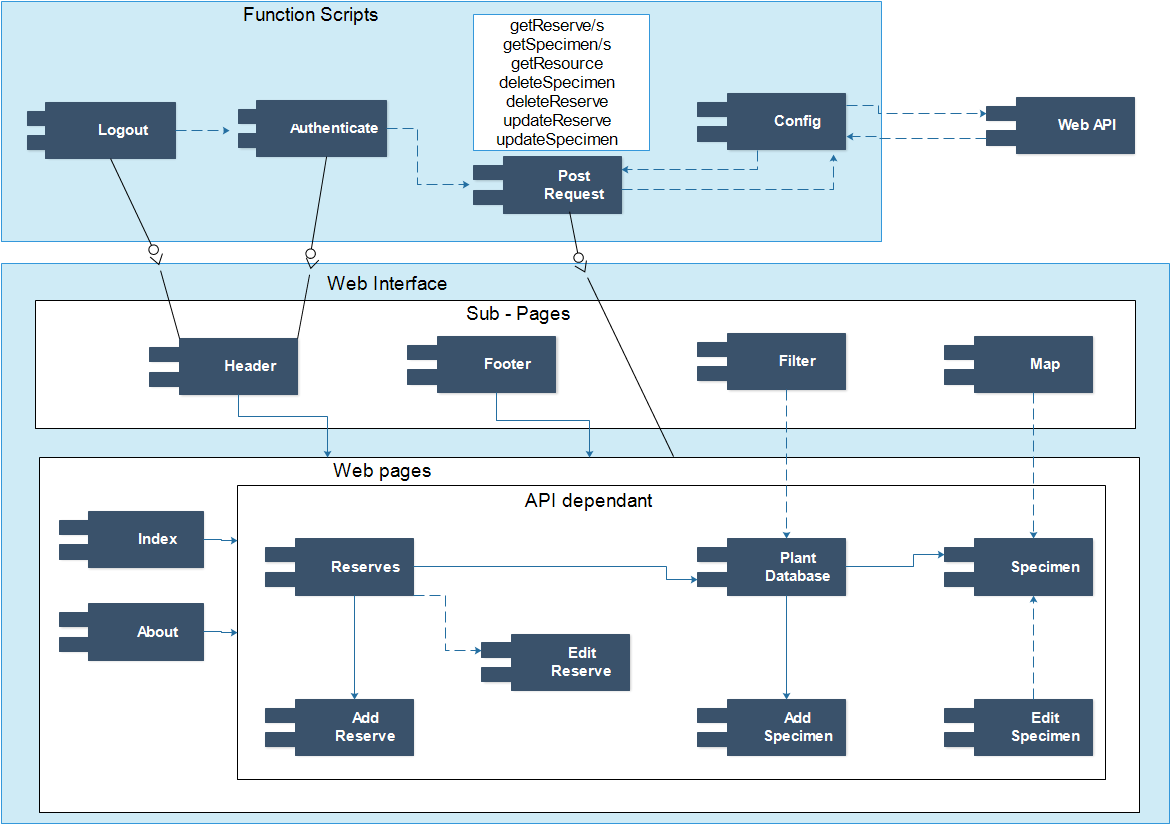
\includegraphics[scale=0.75]{web/webComponentDiagram.png}
        \caption{Web component Diagram}
        \label{fig:webComponentDiagram}
    \end{figure}
\end{landscape}


